\chapter{Operazioni Multiciclo (Multicycle Operations)}

\section{Introduzione alle Operazioni Floating-Point}
Nei capitoli precedenti abbiamo analizzato la pipeline per le istruzioni intere e abbiamo visto come risolvere problemi relativi ai conflitti (hazards) tramite tecniche come il forwarding o modifiche architetturali (es. spostamento del calcolo del salto). 

Quando però introduciamo istruzioni per la gestione dei numeri reali (rappresentati in virgola mobile tramite lo standard IEEE 754), la situazione si complica notevolmente. Le unità \textit{Floating-Point} (FP) devono eseguire operazioni molto più complesse rispetto a quelle intere. Banalmente, una moltiplicazione in virgola mobile richiede non solo la moltiplicazione delle mantisse, ma anche la somma degli esponenti e successive normalizzazioni.

Per gestire questa complessità e forzare queste unità a completare il loro lavoro in un singolo ciclo di clock, il progettista hardware si troverebbe di fronte a due scelte estreme:
\begin{itemize}
    \item utilizzare un clock estremamente lento (penalizzando le istruzioni semplici);
    \item creare unità hardware gigantesche e incredibilmente complesse.
\end{itemize}

Poiché entrambe le soluzioni sono inefficienti (un'area di silicio troppo grande o prestazioni generali degradate), l'alternativa comunemente adottata è permettere alle operazioni FP di richiedere \textbf{più di un ciclo di clock} per completare l'esecuzione. In questa architettura, lo stadio di \textit{Execute} (EX) non è più un blocco monolitico, ma è composto da diverse unità funzionali e viene ripetuto o iterato tante volte quanto richiesto dalla specifica istruzione.

\section{Estensione della Pipeline per il Floating-Point}
La pipeline classica per gli interi è composta dai classici 5 stadi: IF (Instruction Fetch), ID (Instruction Decode), EX (Execute), MEM (Memory access) e WB (Write Back). 

Per supportare le operazioni multiciclo, la fase EX viene espansa in parallelo con moduli dedicati.

% FIGURA DA INSERIRE QUI
% Fonte: Slide 3 e 4 ("Extension for FP")
% Descrizione: Diagramma a blocchi della pipeline espansa. Si vedono IF e ID che si diramano verso 4 unità funzionali parallele: Integer Unit, FP/integer multiply, FP adder, FP/integer divider. Le unità convergono poi verso MEM e WB.
\begin{figure}[H]
    \centering
    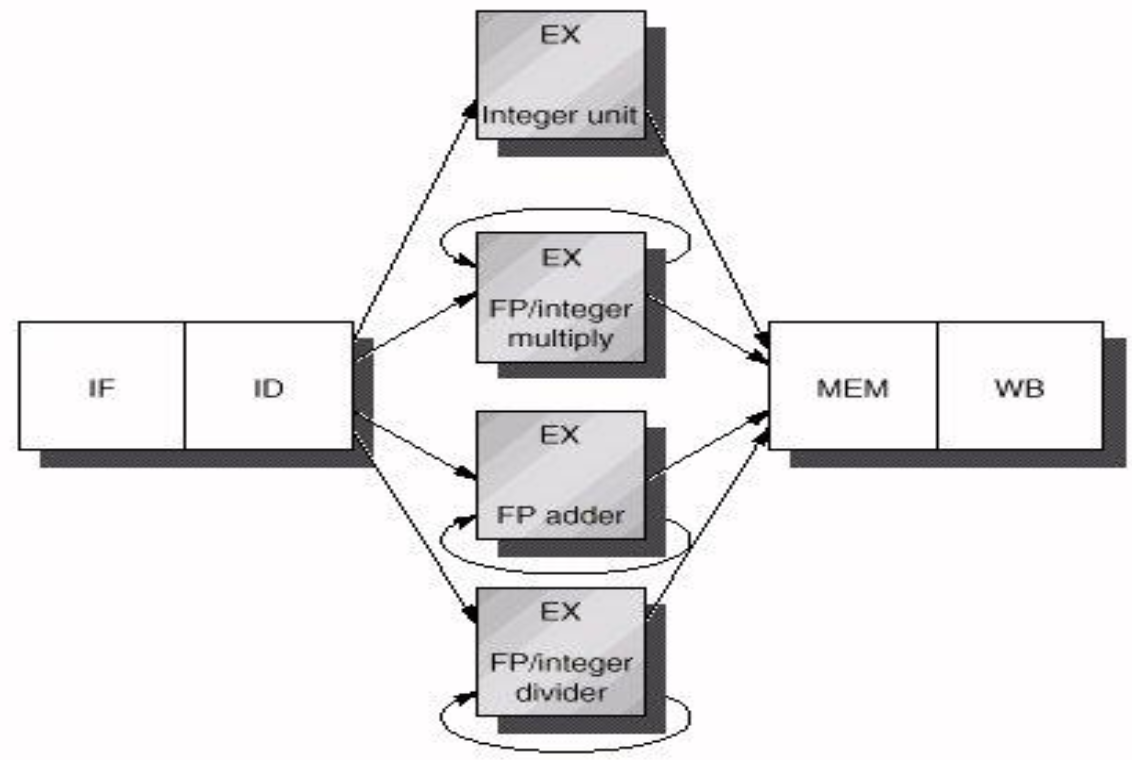
\includegraphics[width=0.8\textwidth]{capitoli/06_pipelining_multicycle/images/fp_pipeline_extension.png}
    \caption{Estensione della pipeline per supportare le operazioni Floating-Point.}
    \label{fig:fp_pipeline_extension}
\end{figure}

Come si nota dallo schema, dopo la fase di decodifica (ID), l'istruzione viene indirizzata all'unità funzionale appropriata. Alcune di queste unità (come l'addizionatore o il moltiplicatore FP) possiedono dei "cicli" (loop) su se stesse, a indicare che il dato permane all'interno dell'unità per più cicli di clock prima di passare alla fase MEM.

\section{Latenza e Intervallo di Inizializzazione}
Per definire il comportamento di queste nuove unità funzionali che richiedono più di un ciclo, dobbiamo introdurre due concetti fondamentali.

\begin{definition}[Latenza]
È il numero di cicli di clock che devono intercorrere tra un'istruzione che produce un risultato e un'istruzione successiva che utilizza quello stesso risultato.
\end{definition}

\begin{remark}
Nella pipeline intera classica, grazie alla rete di \textit{forwarding} (che porta il dato dalla fine della fase EX direttamente all'inizio della nuova fase EX), abbiamo di fatto "azzerato" la latenza. Nel caso del Floating-Point, a causa dell'elaborazione più lunga, il dato non sarà subito disponibile e la latenza tornerà a essere un fattore limitante.
\end{remark}

\begin{definition}[Intervallo di Inizializzazione (Initiation Interval)]
È il numero di cicli di clock che devono trascorrere tra l'avvio (issue) di due operazioni dello stesso tipo indirizzate alla medesima unità funzionale.
\end{definition}

Per comprendere meglio, osserviamo un tipico esempio dei tempi richiesti dalle varie unità.

\begin{table}[H]
    \centering
    \begin{tabular}{lcc}
        \toprule
        \textbf{Functional Unit} & \textbf{Latency} & \textbf{Initiation Interval} \\
        \midrule
        Integer ALU & 0 & 1 \\
        Data Memory & 1 & 1 \\
        FP add & 3 & 1 \\
        FP/integer multiply & 6 & 1 \\
        FP/integer divide & 24 & 25 \\
        \bottomrule
    \end{tabular}
    \caption{Esempio di Latenze e Intervalli di Inizializzazione.}
    \label{tab:latency_example}
\end{table}

\subsection{Unità Pipelined e Non Pipelined}
Guardando la Tabella \ref{tab:latency_example}, possiamo dedurre una caratteristica architetturale cruciale:
\begin{itemize}
    \item \textbf{Unità Pipelined (es. FP add, FP multiply):} Hanno un intervallo di inizializzazione pari a 1. Questo significa che, sebbene l'operazione richieda più cicli per concludersi (es. 4 cicli per la somma, divisi in stadi A1, A2, A3, A4), la struttura interna è a sua volta segmentata in pipeline. Possiamo quindi inserire una nuova somma a ogni ciclo di clock.
    \item \textbf{Unità Non Pipelined (es. FP divide):} L'intervallo di inizializzazione è maggiore o uguale alla latenza (es. 25). Questo significa che l'unità di divisione non è segmentata in stadi indipendenti: una volta avviata una divisione, l'unità è "occupata" per l'intera durata del calcolo. Bisogna attendere che finisca prima di potergliene inviare un'altra.
\end{itemize}

% FIGURA DA INSERIRE QUI
% Fonte: Slide 7/8 ("Pipelined FP units")
% Descrizione: Pipeline con l'esploso degli stadi in EX. Si vede il moltiplicatore diviso in stadi da M1 a M7, l'addizionatore in A1-A4, mentre il blocco DIV è un unico blocco monolitico tratteggiato.
\begin{figure}[H]
    \centering
    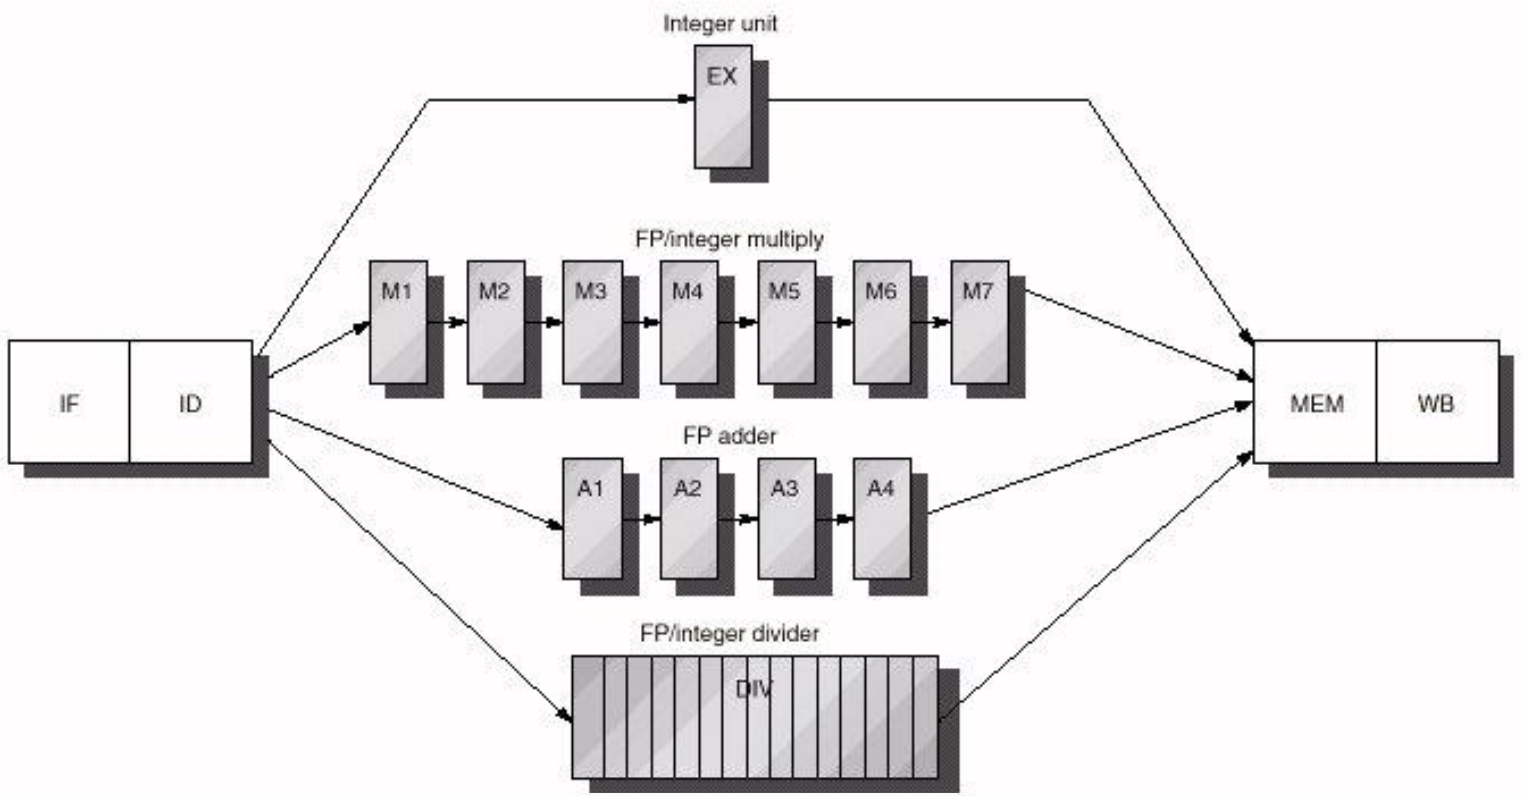
\includegraphics[width=0.9\textwidth]{capitoli/06_pipelining_multicycle/images/fp_pipelined_units.png}
    \caption{Dettaglio degli stadi interni delle unità funzionali (Multiply e Add sono pipelined, Divide non lo è).}
    \label{fig:fp_pipelined_units}
\end{figure}

\section{Conflitti (Hazards) nelle Pipeline Multiciclo}
A causa della struttura eterogenea dello stadio EX, la frequenza dei conflitti (hazards) aumenta significativamente. Il processore cercherà di eseguire (eseguire il \textit{fetch}) un'istruzione a ogni colpo di clock, ma dovrà ritardare la pipeline quando le condizioni non lo permettono.

\subsection{Conflitti Strutturali (Structural Hazards)}
I conflitti strutturali si verificano in due situazioni principali introdotte dalle operazioni multiciclo:
\begin{enumerate}
    \item \textbf{Condivisione di unità non pipelined:} Se due istruzioni indipendenti di divisione (es. la prima divide \texttt{F2/F3} e la seconda \texttt{F5/F6}) arrivano ravvicinate, la seconda dovrà stallare nello stadio di decodifica (ID) perché l'unità DIV è tenuta occupata dalla prima istruzione.
    \item \textbf{Conflitti sul Register File (Scritture simultanee):} Poiché le istruzioni hanno tempi di esecuzione diversi, è possibile che istruzioni partite in momenti diversi terminino esattamente nello stesso ciclo di clock. Se la pipeline possiede un'unica porta di scrittura (Write port) verso il Register File, non sarà in grado di gestire più di un'operazione di \textit{Write Back} (WB) nello stesso ciclo. Il processore dovrà inserire degli stalli per sequenzializzare le scritture.
\end{enumerate}

\begin{figure}[H]
    \centering
    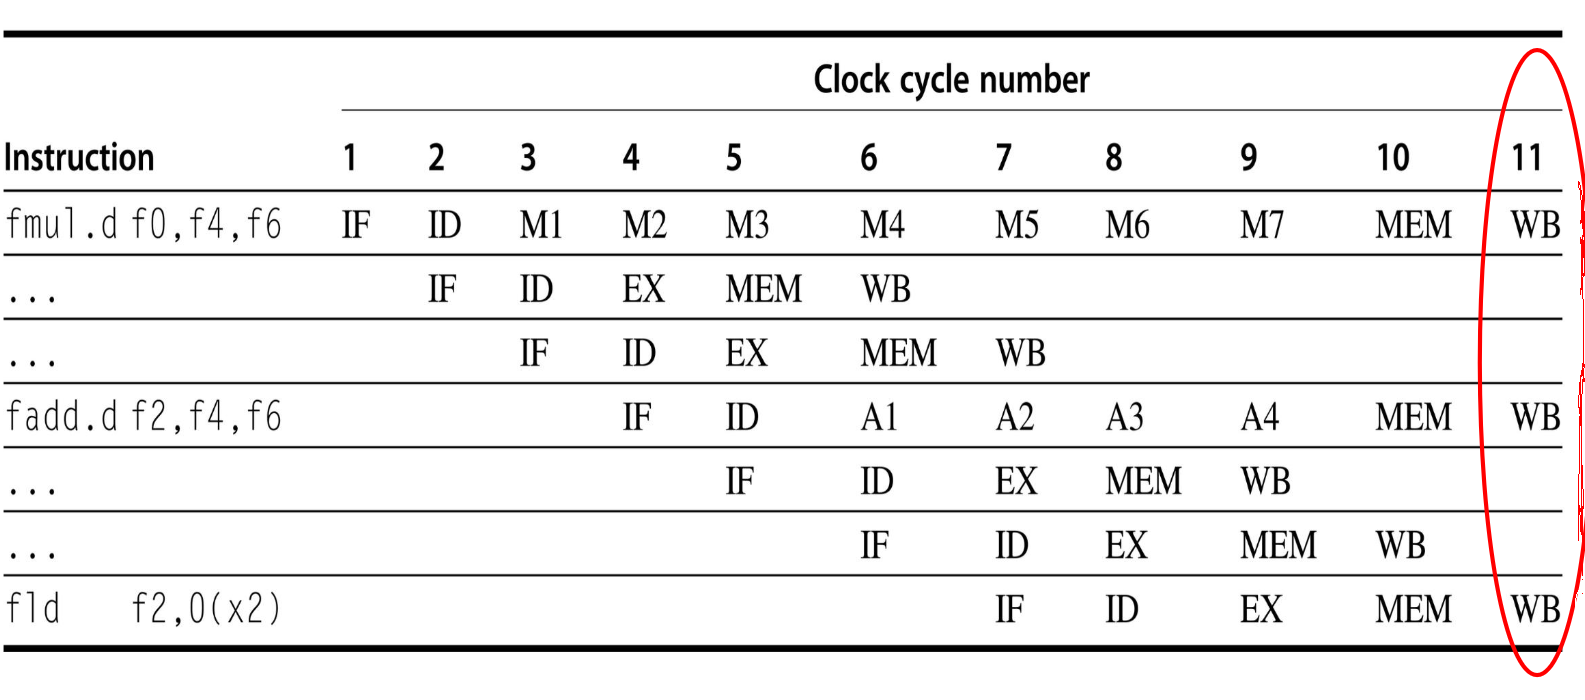
\includegraphics[width=0.8\textwidth]{capitoli/06_pipelining_multicycle/images/register_file_hazards.png}
    \caption{Esempio di conflitti strutturali dovuti a scritture simultanee sul Register File.}
    \label{fig:register_file_hazards}
\end{figure}

\subsection{Conflitti Dati e Forwarding}
Quando due istruzioni Floating-Point sono dipendenti tra loro (la seconda utilizza il risultato della prima), il meccanismo di forwarding deve essere riadattato.

\begin{example}
Sintassi delle operazioni in virgola mobile (es. architettura RISC-V/MIPS): \texttt{fmul.d} indica una moltiplicazione per numeri double (64 bit), mentre \texttt{fmul.s} indica single precision (32 bit).

Supponiamo di avere due moltiplicazioni dipendenti:
\begin{align*}
    &\text{1. } \texttt{fmul.d \quad F1, F2, F3} \quad \text{(Scrive in F1)}\\
    &\text{2. } \texttt{fmul.d \quad F4, F1, F5} \quad \text{(Legge F1)}
\end{align*}
La seconda istruzione non può procedere. Verrà bloccata nella fase di decodifica (ID) finché la prima istruzione non raggiunge l'ultimo stadio della sua esecuzione (es. M7). A quel punto, il risultato potrà subire un \textit{forwarding} verso il primo stadio di esecuzione (M1) della seconda istruzione. 
In questo nuovo scenario, le reti di forwarding diventano molto più complesse, poiché vi sono "molti più sorgenti di dato e molte più destinazioni di dato" rispetto all'architettura per interi.
\end{example}

\begin{remark}
Se le istruzioni \textit{non} sono dipendenti (es. due moltiplicazioni su registri diversi), la seconda istruzione segue normalmente la prima nella pipeline. Entrerà nello stadio M1 non appena la prima passa allo stadio M2, garantendo così una perfetta parallelizzazione del calcolo.
\end{remark}

\section{Moduli e Fasi Operative del Floating-Point}
L'unità FP, data la sua complessità, può essere logicamente scomposta in 8 stadi funzionali base, che vengono ricombinati a seconda dell'operazione.

\begin{table}[H]
    \centering
    \begin{tabular}{cll}
        \toprule
        \textbf{Stage} & \textbf{Functional Unit} & \textbf{Description} \\
        \midrule
        \textbf{A} & Adder & Mantissa ADD stage \\
        \textbf{D} & Divider & Divide \\
        \textbf{E} & Multiplier & Exception test \\
        \textbf{M} & Multiplier & Multiplier I \\
        \textbf{N} & Multiplier & Multiplier II \\
        \textbf{R} & Adder & Rounding \\
        \textbf{S} & Adder & Operand shift \\
        \textbf{U} & (N/A) & Unpack numbers \\
        \bottomrule
    \end{tabular}
    \caption{Componenti di base dell'unità Floating-Point.}
    \label{tab:fp_stages}
\end{table}

Questi blocchi compongono le varie istruzioni. Ad esempio, una somma FP (Add, subtract) passerà per gli stadi di Unpack, Shift, Add e Rounding. 

\begin{remark}[Ottimizzazione della Latenza]
La latenza effettiva per l'uso del dato può essere ridotta di un ciclo di clock (latenza - 1) se l'istruzione di destinazione (quella che attende il dato) non è un'operazione aritmetica, bensì un'istruzione di memorizzazione (\textit{Store instruction}, es. \texttt{fsd}). Questo perché la Store necessita del dato in ingresso solo allo stadio MEM, non in EX.
\end{remark}

\section{Prestazioni (Performance)}
Introdurre istruzioni che richiedono così tanti cicli di clock ha un impatto visibile sul \textit{Cycles Per Instruction} (CPI) medio della macchina.


Dall'analisi delle prestazioni si evince che il comportamento del processore cambia drasticamente in base alla natura del programma eseguito:
\begin{itemize}
    \item \textbf{Programmi Interi:} La causa predominante di decadimento delle prestazioni (aumento del CPI) sono i ritardi legati ai salti (\textit{Branch delays}).
    \item \textbf{Programmi Floating-Point:} Le cause principali di stallo diventano i conflitti sui dati FP (\textit{FP result stalls}, dovuti all'alta latenza delle operazioni) e, in misura minore, i conflitti strutturali.
\end{itemize}
A seconda del programma, il CPI totale può variare ampiamente in un range compreso tra 1.2 e 2.8.